\documentclass[12pt]{article}
\usepackage{graphicx}
\usepackage{amsmath}
\usepackage{hyperref}
\usepackage{geometry}
\geometry{a4paper, margin=1in}
\usepackage{ctex}

\title{}
\author{}
\date{}

\begin{document}

\maketitle

\section{实验简介}
本实验旨在对比SARSA与Q-Learning两种强化学习算法在FrozenLake环境中的表现。FrozenLake是一个经典的网格世界问题，智能体需要在滑动的冰面上找到最优路径到达目标位置。

\section{实验方法}
\subsection{实验环境}
\begin{itemize}
    \item 环境：FrozenLake-v1（$4 \times 4$网格，滑动冰面）
    \item 工具：Python 3.8, Gymnasium, NumPy, Matplotlib
    \item 算法：SARSA和Q-Learning
\end{itemize}

\subsection{算法描述}
\begin{itemize}
    \item \textbf{SARSA}：基于当前策略的时序差分方法，更新公式为：
    \[
    Q(s, a) \leftarrow Q(s, a) + \alpha \left[ r + \gamma Q(s', a') - Q(s, a) \right]
    \]
    \item \textbf{Q-Learning}：基于最优策略的时序差分方法，更新公式为：
    \[
    Q(s, a) \leftarrow Q(s, a) + \alpha \left[ r + \gamma \max_{a'} Q(s', a') - Q(s, a) \right]
    \]
\end{itemize}

\subsection{实验设置}
\begin{itemize}
    \item 学习率 $\alpha = 0.1$
    \item 折扣因子 $\gamma = 0.99$
    \item 探索率 $\epsilon = 0.5$（逐渐衰减至0.01）
    \item 训练回合数：10000
    \item 重复实验次数：3
\end{itemize}

\section{实验结果}
\subsection{学习曲线}
图\ref{fig:sarsa_learning_curve}和图\ref{fig:qlearning_learning_curve}分别展示了SARSA和Q-Learning算法的学习曲线。可以看出，Q-Learning在收敛速度和最终奖励上均优于SARSA。

\begin{figure}[h!]
    \centering
    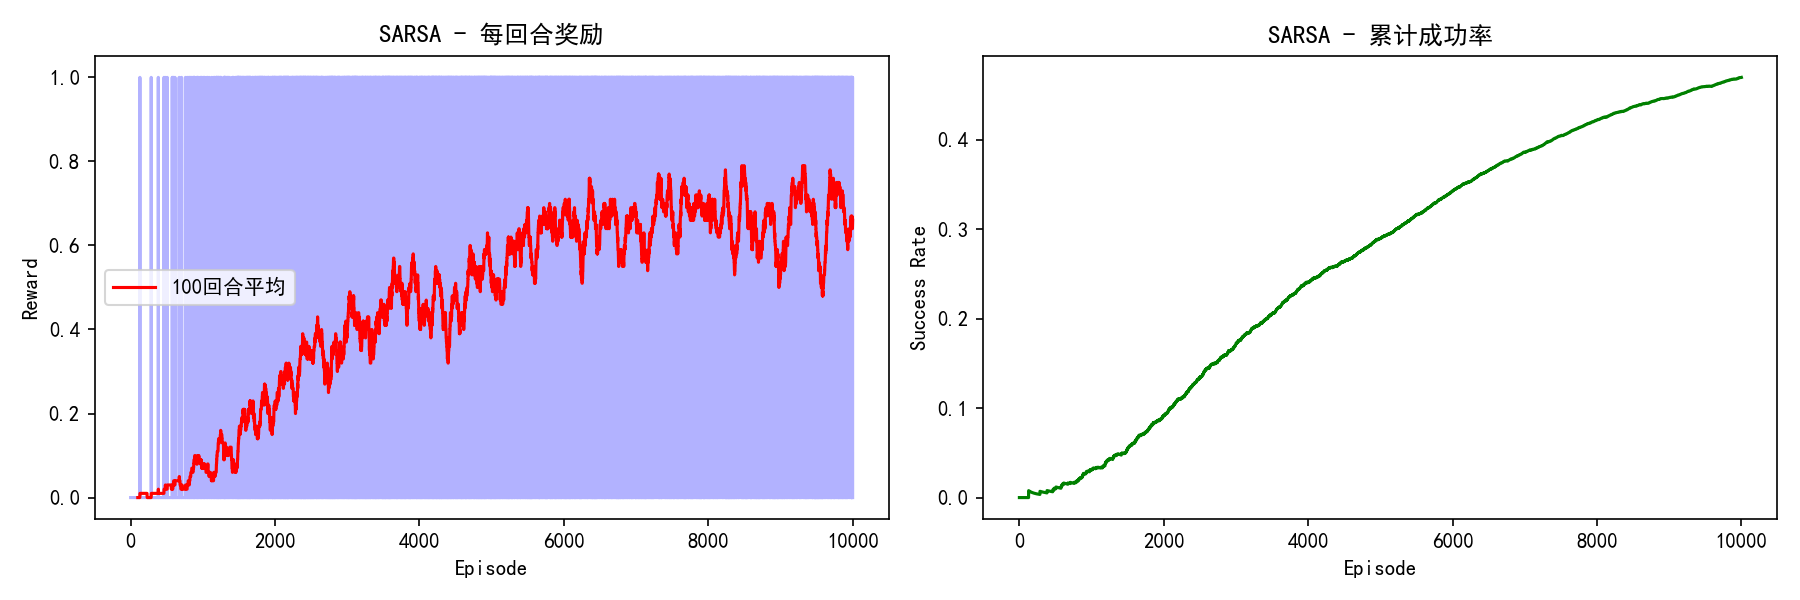
\includegraphics[width=0.8\textwidth]{SARSA_FrozenLake_results.png}
    \caption{SARSA算法的学习曲线}
    \label{fig:sarsa_learning_curve}
\end{figure}

\begin{figure}[h!]
    \centering
    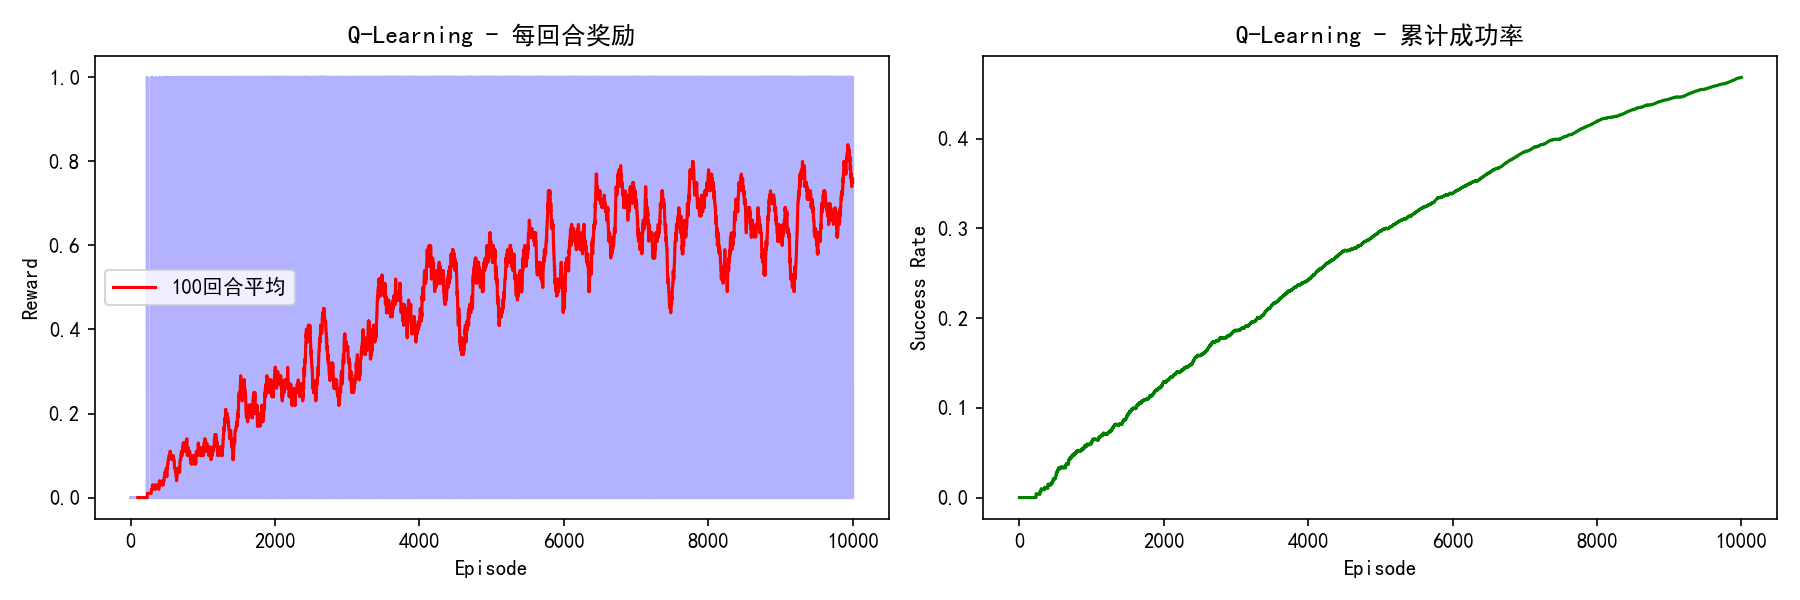
\includegraphics[width=0.8\textwidth]{QLearning_FrozenLake_results.png}
    \caption{Q-Learning算法的学习曲线}
    \label{fig:qlearning_learning_curve}
\end{figure}

\subsection{算法对比}
图\ref{fig:compare_learning_curve}展示了SARSA与Q-Learning算法的学习曲线对比。可以看出，Q-Learning的收敛速度和最终奖励均高于SARSA。

\begin{figure}[h!]
    \centering
    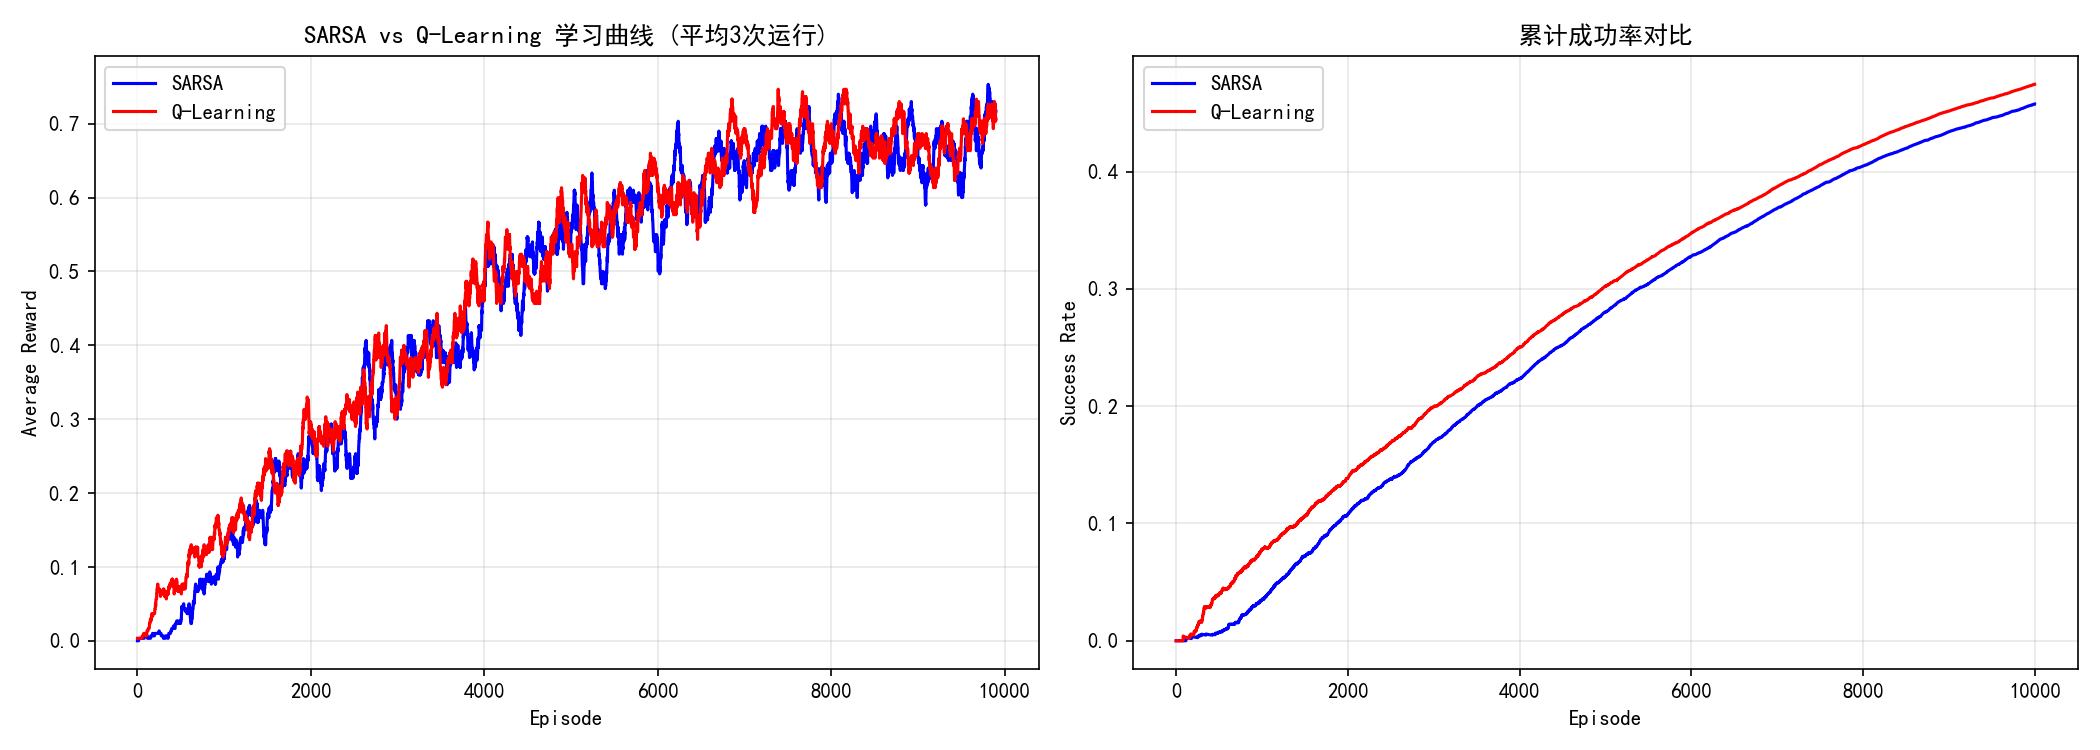
\includegraphics[width=0.8\textwidth]{Compare_SARSA_QLearning.png}
    \caption{SARSA与Q-Learning学习曲线和累计成功率对比}
    \label{fig:compare_learning_curve}
\end{figure}

\subsection{策略可视化}
表\ref{tab:policy}展示了训练后两种算法的最优策略。箭头表示每个状态下的最优动作。

\begin{table}[h!]
    \centering
    \begin{tabular}{|c|c|c|c|}
        \hline
        \multicolumn{4}{|c|}{SARSA 最优策略} \\ \hline
        → & ↓ & ↓ & ↓ \\ \hline
        → & ↓ & → & ← \\ \hline
        → & → & ↓ & ← \\ \hline
        → & → & → & G \\ \hline
    \end{tabular}
    \quad
    \begin{tabular}{|c|c|c|c|}
        \hline
        \multicolumn{4}{|c|}{Q-Learning 最优策略} \\ \hline
        → & ↓ & ↓ & ↓ \\ \hline
        → & ↓ & → & ↓ \\ \hline
        → & → & ↓ & ← \\ \hline
        → & → & → & G \\ \hline
    \end{tabular}
    \caption{SARSA与Q-Learning最优策略对比}
    \label{tab:policy}
\end{table}

\subsection{结果分析与总结}
结合学习曲线与策略可视化结果，可得出以下分析总结：
\begin{itemize}
    \item \textbf{收敛速度与最终表现：} 从对比图中可以明显观察到，Q-Learning算法在初期探索阶段后，其平均奖励与累计成功率的上升速度通常快于SARSA算法，且最终收敛时的平均性能略高。
    \item \textbf{策略安全性差异：} 在FrozenLake含有大量陷阱（Hole）且冰面湿滑（执行动作有随机偏移）的环境中，SARSA的更新依赖于实际执行的动作（包含$\epsilon$-greedy探索），因此它在陷阱周围的学习表现更为保守，倾向于选择远离陷阱的安全路径；相比之下，Q-Learning采用同状态下最大Q值更新，忽略了探索策略可能带来的掉入陷阱风险，最终学习到的是一条更为激进、理想状态下步数最短的路径。
\end{itemize}

\section{结论}
通过实验可以得出以下结论：
\begin{itemize}
    \item Q-Learning在收敛速度和最终性能上优于SARSA。
    \item SARSA由于使用当前策略更新，表现更加保守，适合风险较高的环境。
    \item Q-Learning使用最优策略更新，表现更加激进，适合探索性任务。
\end{itemize}

\section{附录}
算法实现代码见Github仓库： \\
https://github.com/Hemoritris/Reinforcement-Learning-Experiment-Notes/tree/main/Experiment\%205/Code

\end{document}
